\documentclass{standalone}
\usepackage{amssymb,amsmath,latexsym, braket}
\usepackage{tikz, pgfplots, graphicx}
\begin{document}
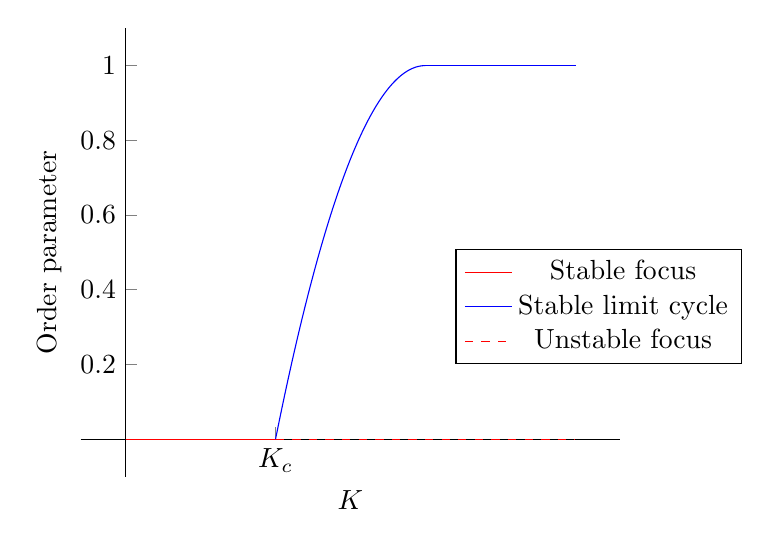
\begin{tikzpicture}
    \begin{axis}[domain=0:4,legend style={at={(axis cs:2.2,0.2)},anchor=south west},
    axis lines*=middle,
    xlabel=$K$,
    ylabel=Order parameter,
	xtick={1},
	xticklabel={$K_c$},
    %axis lines = middle,
%every axis x label/.style={at={(current axis.right of origin)},anchor=west},
%every axis y label/.style={at={(current axis.north west)},above=2mm},
     ]
    \addplot[samples=200, mark=none,domain=0:1, color=red] {0};
    \addplot[samples=200, mark=none,domain=1:2, color=blue,line legend] {-(x-2)*(x-2)+1};
    \addplot[samples=200, mark=none,domain=2:3, color=blue,forget plot] {1};
    \addplot[samples=200, mark=none,domain=1:3, color=red, line legend,dashed] {0};
    \legend{Stable focus, Stable limit cycle, Unstable focus};
    \end{axis}
\end{tikzpicture}
\end{document}